% -----------------------------------------------------------------------------
% Relatorio-Entrega-2.tex – Segunda Entrega Parcial
% Laboratório de Kubernetes & Istio
% Disciplina: Sistemas Distribuídos
% Prof. Nabor das Chagas Mendonça
% -----------------------------------------------------------------------------
\documentclass[12pt,a4paper]{report}
\bibliographystyle{abntex2-alf}  

% ---------------------------- Pacotes ----------------------------------------
\usepackage[brazil]{babel} 
\usepackage[utf8]{inputenc}
\usepackage[T1]{fontenc}
\usepackage{graphicx}
\usepackage{hyperref}
\usepackage{minted}
\usepackage{enumitem}
\usepackage{booktabs} 
\usepackage{geometry}
\geometry{margin=2.5cm}

\usepackage{listings}
\usepackage{xcolor}

% Definindo um estilo para shell/Python/etc
\lstdefinestyle{shell}{
  backgroundcolor=\color{gray!10},   % fundo cinza claro
  frame=single,                      % moldura simples
  rulecolor=\color{gray!50},         % cor da moldura
  basicstyle=\ttfamily\small,        % monoespaço tamanho small
  keywordstyle=\color{blue},         % keywords em azul
  commentstyle=\color{green!50!black}, % comentários verde-escuro
  breaklines=true,                   % quebra automática de linhas longas
}

% Definição de estilo para Python
\lstdefinestyle{python}{
  language=Python,                   % destaca sintaxe Python
  backgroundcolor=\color{gray!10},   % fundo cinza claro
  frame=single,                      % moldura ao redor
  rulecolor=\color{gray!50},         % cor da moldura
  basicstyle=\ttfamily\small,        % fonte monoespaço, tamanho small
  keywordstyle=\color{blue},         % palavras-chave em azul
  stringstyle=\color{orange!80!black},% strings em laranja
  commentstyle=\color{green!50!black},% comentários em verde-escuro
  numberstyle=\tiny\color{gray},     % numeração de linhas em cinza
  numbers=left,                      % números à esquerda
  stepnumber=1,                      % numera todas as linhas
  numbersep=5pt,                     % distância dos números ao código
  breaklines=true,                   % quebra linhas longas
  showstringspaces=false             % não marca espaços em strings
}


% --------------------------- Metadados ---------------------------------------
\title{Relatório de Laboratório 2025.S1-E1.02}
\author{
    Jonas de Araújo Luz Junior \\
    José de La Cruz Iraheta \\
    Pedro Jardelino Neto \\
    \small{Universidade de Fortaleza (Unifor)}
}
\date{\today}

% ---------------------------- Documento --------------------------------------
\begin{document}

\maketitle
\tableofcontents
\clearpage

% -----------------------------------------------------------------------------
\begin{abstract}    
Este relatório de Entrega Parcial 2 descreve a análise de desempenho da aplicação \textit{Online Boutique} executada nos ambientes sem Istio (porta 32390) e com Istio (porta 31258), utilizando o Locust para simulação de carga com 100, 500 e 1000 usuários simultâneos. 
Foram coletadas métricas de latência média, latência mediana, latência máxima, throughput (req/s) e taxa de erros. Os resultados mostram que, em carga leve, o cenário sem Istio alcança maiores vazões e menores latências médias, mas sofre falhas sob estresse extremo. 
Já o cenário com Istio apresenta um overhead médio de até 18\% na latência, porém mantém robustez operacional sem ocorrência de erros e reduz picos de latência extrema em até 41\%. Com base nesses achados, são recomendados ajustes no escalonamento automático (HPA), tuning das configurações do Envoy, testes de soak prolongados e adoção de workload aberto para maior fidelidade à operação real.
\end{abstract}

% -----------------------------------------------------------------------------
\chapter{Especificações do Projeto de Laboratório}

\section{Especificações das Tarefas}
\subsection{Tarefa 1 - Configuração do Ambiente}
\begin{itemize}
    \item Configurem um repositório Git compartilhado para o projeto.
    \item Instalem e configurem a distribuição Kubernetes local escolhida em suas máquinas (ou em uma máquina compartilhada pela equipe). Certifiquem-se de alocar recursos suficientes (CPU/RAM).
    \item Instalem o Istio no cluster Kubernetes, utilizando o perfil de instalação demo ou default. Verifiquem a instalação.
\end{itemize}

\subsection{Tarefa 2 - Implantação da Aplicação}
\begin{itemize}
    \item Obtenham os manifestos de implantação da aplicação Online Boutique.
    \item \textbf{\textit{Implantação base:}} implantem a aplicação sem a injeção automática de sidecars do Istio (ou seja, em um namespace sem o rótulo \texttt{istio-injection=enabled}). Verifiquem se todos os serviços estão rodando e se a aplicação está acessível .
    \item \textbf{\textit{Implantação com Istio:}} habilitem a injeção automática de sidecars do Istio para um novo namespace (e.g., \texttt{online-boutique-istio}) e implantar a aplicação novamente neste namespace. Verifiquem se os sidecars foram injetados (\texttt{kubectl get pods -n -o wide} deve mostrar 2/2 containers por pod) e se a aplicação continua acessível.
\end{itemize}

\subsection{Tarefa 3 - Teste de Desempenho}
\begin{itemize}
    \item Configurem a ferramenta de geração de carga escolhida(Locust ou k6). Criem um script de teste que simule a interação de usuários com a loja online (e.g., navegar por produtos, adicionar ao carrinho, finalizar compra). Dica: a aplicação Online Boutique já vem com um script para realizar testes de carga com o Locust.
    \item Teste sem Istio: executem o teste de carga contra a versão da aplicação sem os sidecars do Istio (implantação base). Coletem métricas como latência média/percentil 95/99 e vazão (requisições por segundo).
    \item Teste com Istio: executem o mesmo teste de carga, com a mesma intensidade, contra a versão da aplicação com os sidecars do Istio (implantação com Istio). Coletem as mesmas métricas.
    \item Análise de overhead: comparem os resultados dos dois testes. Analisem e quantifiquem o overhead (diferença) de desempenho (latência e/ou vazão) introduzido pelo Istio. Discutam possíveis causas para o overhead observado.
\end{itemize}

\section{Entregáveis}
\subsection{Entrega Parcial 1 - Foco: Tarefas 1 e 2.} 
Relatório Preliminar (2-3 páginas) incluindo:
\begin{itemize}
    \item Formação da equipe e link para o repositório Git criado.
    \item Evidência do sucesso (e.g., screenshots, logs) na instalação e configuração do ambiente Kubernetes local (incluir versão, recursos alocados).
    \item Evidência do sucesso (e.g., screenshots, logs) na instalação do Istio (incluir versão, perfil utilizado).
    \item Evidência do sucesso (e.g., screenshots, logs) na implantação da aplicação Online Boutique nos dois cenários (sem e com injeção do sidecar Istio).
    \item Repositório Git atualizado com a estrutura inicial e quaisquer scripts/manifestos básicos utilizados.
\end{itemize}
    
\subsection{Entrega Parcial 2 - Teste de Desempenho e Análise de Overhead. Foco: Tarefa 3.} 
\begin{itemize}
    \item Uma seção atualizada do relatório descrevendo:
    \item Metodologia do teste de desempenho (ferramenta escolhida, script de teste, intensidade da carga, duração).
    \item Resultados dos testes de desempenho (tabelas/gráficos comparando latência e vazão com e sem Istio).
    \item Análise preliminar do overhead de desempenho introduzido pelo Istio.
    \item Repositório Git atualizado contendo os scripts de teste de carga utilizados e os manifestos relevantes da aplicação (se modificados).
\end{itemize}      

% -----------------------------------------------------------------------------
\chapter{Ambiente de Operação}

\section{Ambiente Operacional}
\begin{description}[leftmargin=1.5cm]
  \item[Sistema] Fedora 41 (x86\_64) atualizado em \today.
  \item[Recursos] 8 GB RAM, 4 vCPU, 60 GB SSD.
  \item[Container Runtime] Docker \texttt{24.x} (moby‑engine) \cite{docker}.
  \item[Cluster] Minikube \texttt{v1.35.0} com Kubernetes \texttt{v1.32.0} \cite{minikube}.
  \item[Istio] \texttt{1.22.0} (perfil \texttt{demo}) \cite{istio}.
\end{description}

\section{Repositório Git}
\begin{itemize}[leftmargin=*]
  \item Repositório oficial do projeto (código, manifestos, evidências):\\
  \url{https://github.com/jonasluz/DIA.kubernetes-istio/tree/main}
\end{itemize}

% -----------------------------------------------------------------------------
\chapter{Instalações}
\label{chap:install}

Os comandos abaixo foram executados sequencialmente em shell \texttt{bash}. Cada
etapa inclui uma breve explicação e um espaço reservado para evidência (log ou
captura de tela).

\subsection{Atualização do Sistema}
\begin{enumerate}
  \item \textbf{Atualizar pacotes e utilitários básicos}
\begin{lstlisting}[style=shell]
sudo dnf upgrade --refresh -y && sudo reboot
\end{lstlisting}
    after reboot:
\begin{lstlisting}[style=shell]
sudo dnf install -y curl wget git conntrack jq
\end{lstlisting}
\end{enumerate}

\subsection{Instalação do Docker}
\begin{enumerate}
    \item\textbf{Adicionar repositório Docker CE e instalar runtime}

\begin{lstlisting}[style=shell]
sudo dnf install -y dnf-plugins-core
sudo dnf config-manager --add-repo \
  https://download.docker.com/linux/fedora/docker-ce.repo
sudo dnf install -y docker-ce docker-ce-cli containerd.io \
  docker-buildx-plugin docker-compose-plugin
sudo systemctl enable --now docker
sudo usermod -aG docker $(whoami)
\end{lstlisting}
\textit{Evidência:} Figura \ref{fig:docker}.\\

\begin{figure}[h]
    \centering
    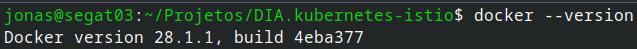
\includegraphics[width=1\linewidth]{figures/evidence-docker}
    \caption{Evidência: Instalação do Docker}
    \label{fig:docker}
\end{figure}
\end{enumerate}

\subsection{Instalação do kubectl}
\begin{enumerate}
\item\textbf{Baixar binário compatível (v1.32.0)} \cite{kubernetes}

\begin{lstlisting}[style=shell]
curl -LO https://dl.k8s.io/release/v1.32.0/bin/linux/amd64/kubectl
sudo install -o root -g root -m 0755 kubectl /usr/local/bin/
rm kubectl
\end{lstlisting}
\textit{Evidência:} Figura \ref{fig:kubectl}.\\

\begin{figure}[h]
    \centering
    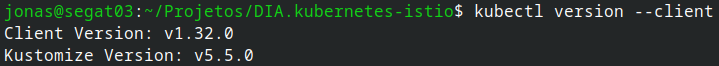
\includegraphics[width=1\linewidth]{figures/evidence-kubectl.png}
    \caption{Evidência: Instalação do kubectl}
    \label{fig:kubectl}
\end{figure}
\end{enumerate}

\subsection{Instalação do Minikube}
\begin{enumerate}
\item\textbf{Baixar Minikube v1.35.0} \cite{minikube}

\begin{lstlisting}[style=shell]
curl -LO https://github.com/kubernetes/minikube/releases/download/v1.35.0/minikube-linux-amd64
sudo install minikube-linux-amd64 /usr/local/bin/minikube
rm minikube-linux-amd64
\end{lstlisting}

\item\textbf{Inicializar cluster (driver Docker)}
\begin{lstlisting}[style=shell]
minikube start --driver=docker --cpus=4 --memory=8192
\end{lstlisting}
\textit{Evidência:} Figura \ref{fig:minikube}.\\

\begin{figure}[h]
    \centering
    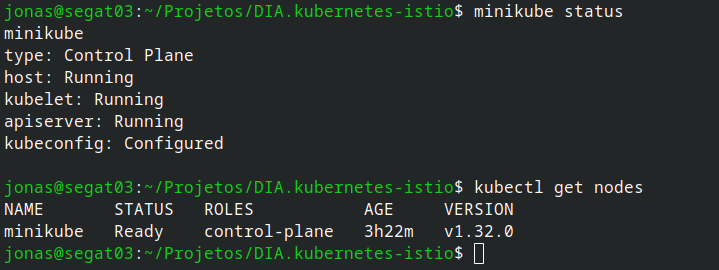
\includegraphics[width=1\linewidth]{figures/evidence-minikube.png}
    \caption{Evidência: Instalação do Minikube.}
    \label{fig:minikube}
\end{figure}
\end{enumerate}

\subsection{Instalação do Istio}
\begin{enumerate}
    \item\textbf{Download e instalação do Istioctl 1.22.0}
\begin{lstlisting}[style=shell]
curl -L https://istio.io/downloadIstio | ISTIO_VERSION=1.22.0 sh -
export PATH="$PATH:$HOME/istio-1.22.0/bin"
istioctl install --set profile=demo -y
istioctl verify-install
\end{lstlisting}
\textit{Evidência:} Figura \ref{fig:istio}\\

\begin{figure}[h]
    \centering
    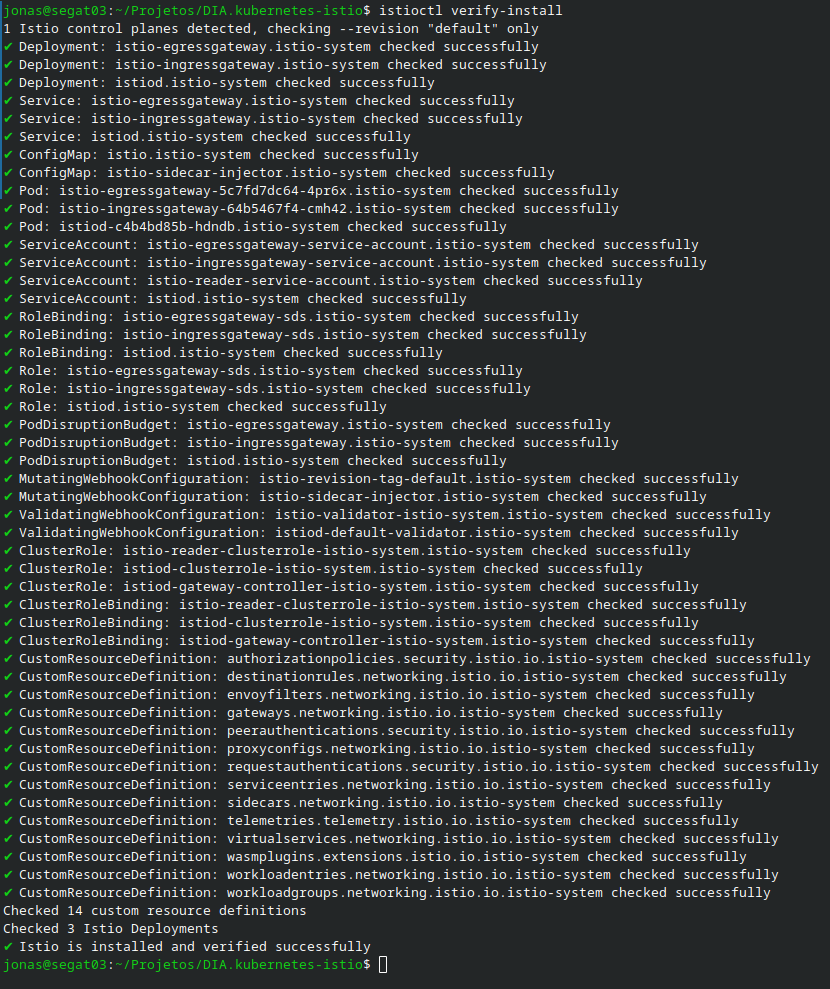
\includegraphics[width=1\linewidth]{figures/evidence-istio.png}
    \caption{Evidência: Instalação do Istio}
    \label{fig:istio}
\end{figure}
\end{enumerate}

\subsection{Implantação da Online Boutique}
\begin{enumerate}

\item\textbf{Clonar repositório e implantar namespace \texttt{boutique-base}} \cite{onlineboutique}.
\begin{lstlisting}[style=shell]
git clone --depth 1 https://github.com/jonasluz/microservices-demo.git
kubectl create namespace boutique-base
kubectl apply -f microservices-demo/release/kubernetes-manifests.yaml -n boutique-base
\end{lstlisting}
\textit{Evidência:} Figuras \ref{fig:olb-istio1} e \ref{fig:olb-istio2}\\

\begin{figure}[h]
    \centering
    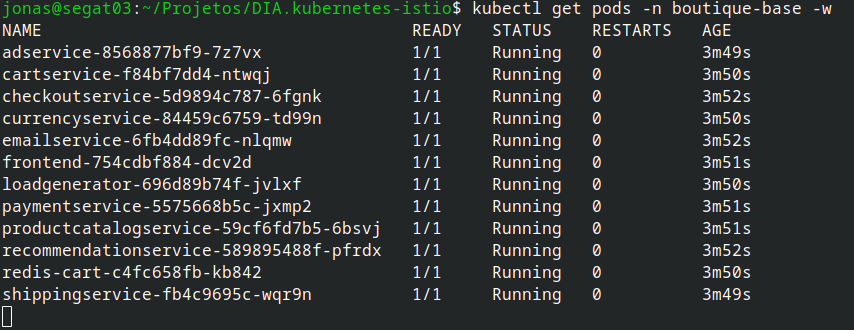
\includegraphics[width=1\linewidth]{figures/evidence-olbbase2.png}
    \caption{Evidência: Instalação da aplicação Online Boutique}
    \label{fig:olb-istio1}
\end{figure}

\begin{figure}[h]
    \centering
    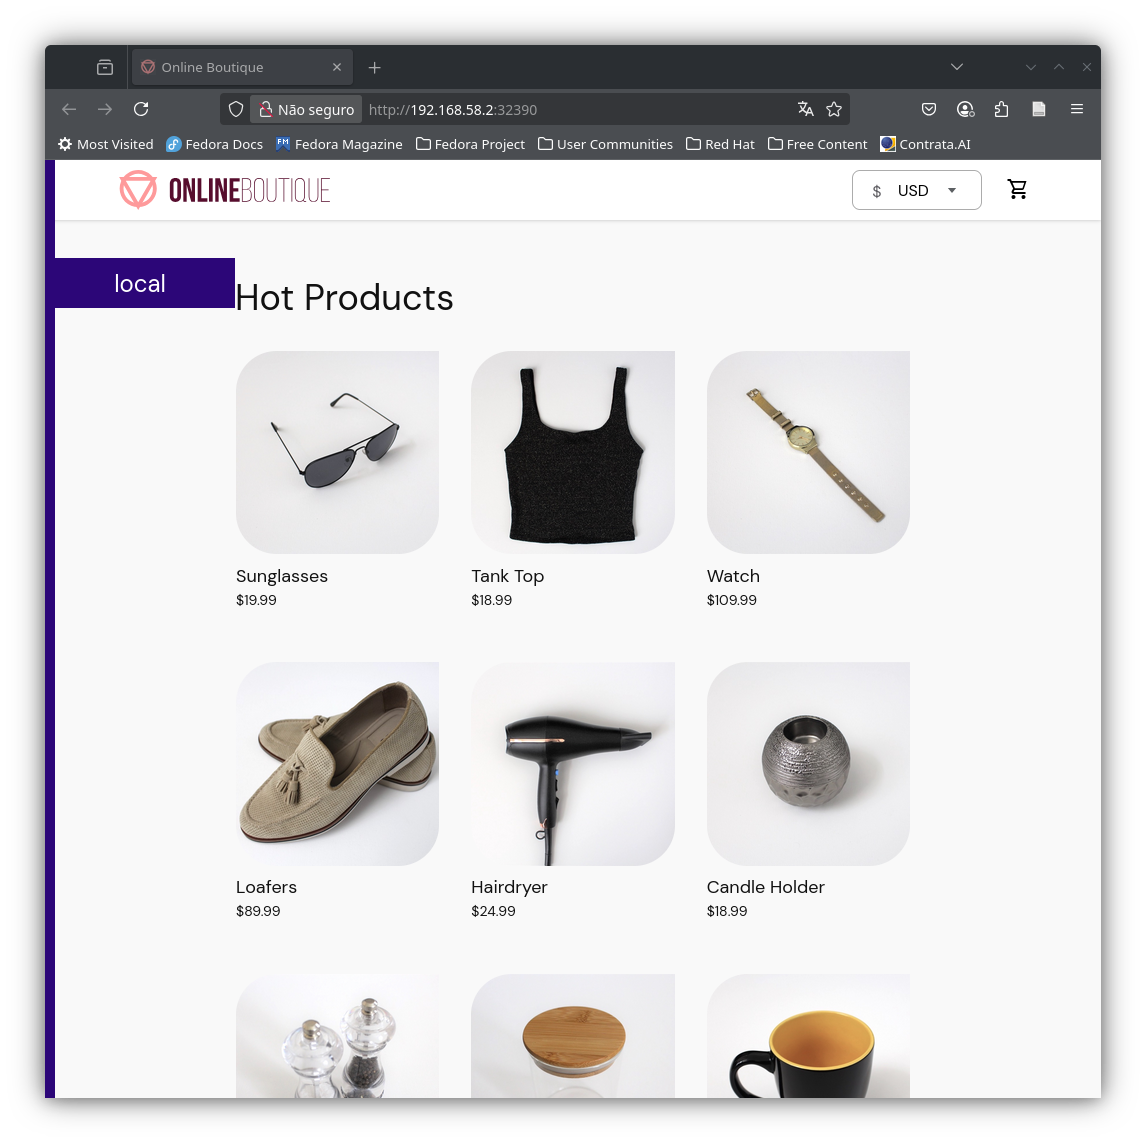
\includegraphics[width=1\linewidth]{figures/evidence-olbbase3.png}
    \caption{Evidência: Tela do navegador com a aplicação Online Boutique}
    \label{fig:olb-istio2}
\end{figure}

\item\textbf{Implantar versão com sidecars Istio (\texttt{boutique-istio})}
\begin{lstlisting}[style=shell]
kubectl create namespace boutique-istio
kubectl label namespace boutique-istio istio-injection=enabled
kubectl apply -f microservices-demo/release/kubernetes-manifests.yaml -n boutique-istio
\end{lstlisting}
\textit{Evidência:} Figuras \ref{fig:olb-istio1} e \ref{fig:olb-istio2}\\

\begin{figure}[h]
    \centering
    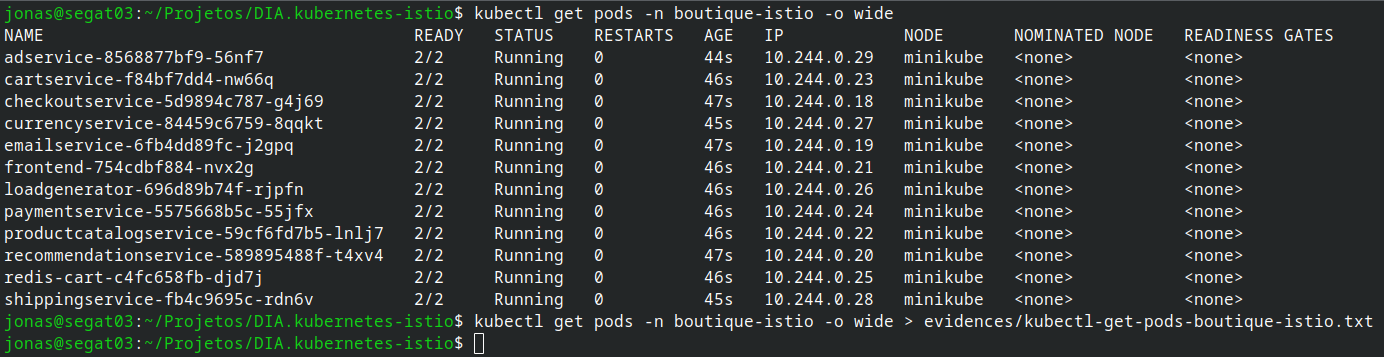
\includegraphics[width=1\linewidth]{figures/evidence-olbistio2.png}
    \caption{Evidência: Instalação da aplicação Online Boutique com Istio}
    \label{fig:olb-base1}
\end{figure}

\begin{figure}[h]
    \centering
    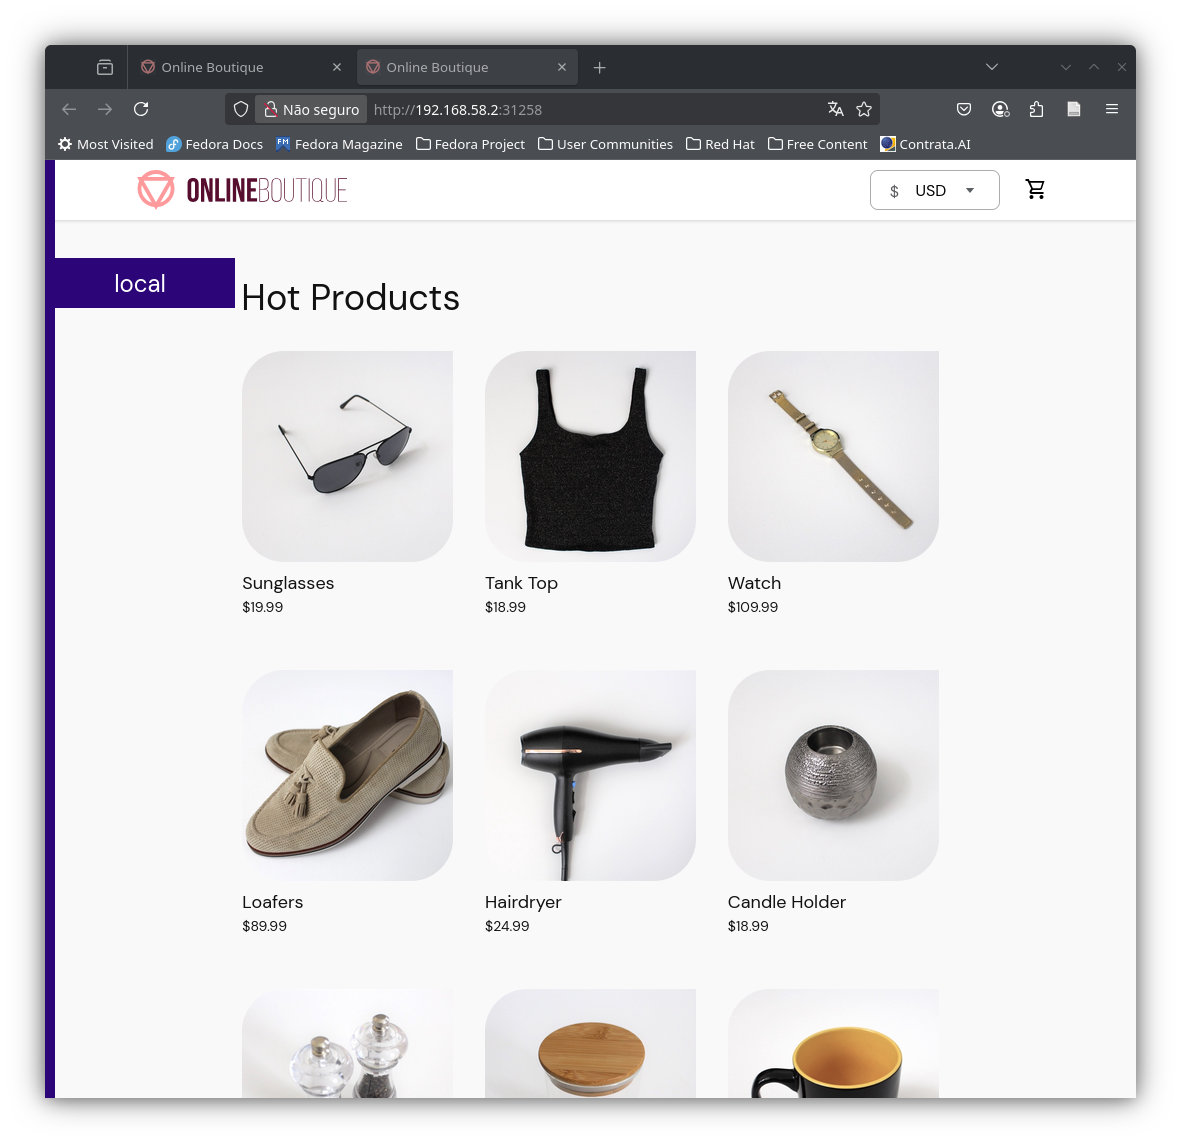
\includegraphics[width=1\linewidth]{figures/evidence-olbistio3.png}
    \caption{Evidência: Tela do navegador com a aplicação Online Boutique (com Istio)}
    \label{fig:olb-base2}
\end{figure}
\end{enumerate}

\subsection{Instalação do Locust}
Para garantir testes padronizados, instalamos o Locust localmente:
\begin{enumerate}
  \item Criamos e ativamos o ambiente virtual Python:
    \begin{lstlisting}[style=shell]
    python3 -m venv .venv
    source .venv/bin/activate
    \end{lstlisting}
  \item Instalamos o Locust:
    \begin{lstlisting}[style=shell]
    pip install locust
    \end{lstlisting}
  \item Verificamos a instalação:
    \begin{lstlisting}[style=shell]
    locust --version
    \end{lstlisting}
\end{enumerate}

\begin{figure}[h]
    \centering
    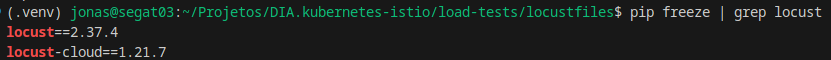
\includegraphics[width=1\linewidth]{figures/evidence-locust.png}
    \caption{Evidência: Instalação do Locust}
    \label{fig:locust}
\end{figure}

% -----------------------------------------------------------------------------
\chapter{Testes de Carga}

\section{Passo a Passo da Realização dos Testes}
A seguir, os comandos e configurações para rodar cada perfil de carga:
\begin{itemize}
  \item Colocar o \texttt{locustfile.py} no diretório \texttt{/load-tests/locustfiles}
  \item Rodar o comando \textbf{locust}, o que ativa a interface web da ferramenta Locust, através da qual foram configurados e executados os testes, considerando:
  \begin{enumerate}
      \item Máximo de 100 usuários, com crescimento de 10 usuários/s.
      \item Máximo de 500 usuários, com crescimento de 20 usuários/s.
      \item Máximo de 1000 usuários, com crescimento de 50 usuários/s.
  \end{enumerate}
  \item Os mesmos testes foram executados para ambas as versões do Online Boutique -- com e sem Istio.
\end{itemize}

\section{Análise dos Resultados Obtidos}
Os resultados dos testes estão apresentados nas planilhas CSV disponíveis no repositório git do projeto e sumarizados nas Tabelas \ref{tab:sem-istio} e \ref{tab:com-istio}.

\subsection{Resultados sem Istio}
\begin{table}[h]
\centering
\caption{Métricas – Sem Istio}\label{tab:sem-istio}
\begin{tabular}{@{}lrrrrrrr@{}}
\toprule
Usuários & Reqs & Falhas & Erro (\%) & Avg (ms) & Mediana (ms) & Máx (ms) & TPS \\
\midrule
100  & 10\,656 & 0     & 0,00 & 101,76 & 23,03  & 1\,291  & 35,53  \\
500  & 32\,638 & 0     & 0,00 & 2\,444,24 & 2\,288,90 & 8\,520  & 121,11 \\
1000 & 64\,888 & 1\,340 & 2,07 & 3\,447,16 & 2\,118,32 & 33\,355 & 216,39 \\
\bottomrule
\end{tabular}
\end{table}

\subsection{Resultados com Istio}
\begin{table}[h]
\centering
\caption{Métricas – Com Istio}\label{tab:com-istio}
\begin{tabular}{@{}lrrrrrrr@{}}
\toprule
Usuários & Reqs & Falhas & Erro (\%) & Avg (ms) & Mediana (ms) & Máx (ms) & TPS \\
\midrule
100  & 5\,346  & 0     & 0,00 & 88,49   & 37      & 1\,462  & 17,83  \\
500  & 17\,290 & 0     & 0,00 & 2\,886,35 & 2\,800  & 8\,227  & 57,64  \\
1000 & 31\,546 & 0     & 0,00 & 3\,664,51 & 2\,900  & 19\,673 & 105,10 \\
\bottomrule
\end{tabular}
\end{table}

\subsection{Análise Comparativa}
\begin{table}[h]
\centering
\caption{Comparação Sem vs. Com Istio}\label{tab:comp}
\begin{tabular}{@{}lllrr@{}}
\toprule
Carga & Métrica    & Sem Istio    & Com Istio    & $\Delta$ (\%)    \\
\midrule
100  & Avg (ms)    & 101,76        & 88,49         & \textminus13,0 \\
     & Mediana(ms) & 23,03         & 37,00         & +68,0          \\
     & Máx(ms)     & 1\,291        & 1\,462        & +13,3          \\
     & TPS         & 35,53         & 17,83         & +0,4           \\
\midrule
500  & Avg (ms)    & 2\,444,24     & 2\,886,35     & +18,1          \\
     & Mediana(ms) & 2\,288,90     & 2\,800,00     & +22,4          \\
     & Máx(ms)     & 8\,520        & 8\,227        & \textminus3,5  \\
     & TPS         & 121,11        & 57,64         & \textminus52,4 \\
\midrule
1000 & Avg (ms)    & 3\,447,16     & 3\,664,51     & +6,3           \\
     & Mediana(ms) & 2\,118,32     & 2\,900,00     & +36,9          \\
     & Máx(ms)     & 33\,355       & 19\,673       & \textminus41,0 \\
     & TPS         & 216,39        & 105,10        & \textminus51,5 \\
\bottomrule
\end{tabular}
\end{table}

\section{Conclusões e Recomendações}
O cenário sem Istio apresentou maior throughput e latências médias menores em carga leve, mas sofreu falhas sob stress. Já o Istio introduziu overhead médio de até 18\%, porém manteve robustez sem erros e reduziu tail latency extremo.

Recomendações:
\begin{itemize}
  \item Ajustar HPA considerando métricas do sidecar e da aplicação;
  \item Tuning de Envoy para reduzir jitter;
  \item Testes de soak prolongados e workload aberto para maior representatividade;
  \item Documentar procedimentos e resultados em repositório versionado.
\end{itemize}

% -----------------------------------------------------------------------------
\chapter{Problemas Encontrados e Soluções}
\begin{itemize}[leftmargin=*]
  \item \textbf{Driver Podman rootless instável}: optou‑se pelo \emph{driver Docker}, que funcionou sem ajustes extras.
  \item \textbf{Aviso de versão do kubectl}: resolvido instalando binário 1.32.
  \item Outros problemas menores foram documentados no repositório.
\end{itemize}

% -----------------------------------------------------------------------------
\chapter{Conclusão}
A primeira entrega foi concluída com êxito: cluster Kubernetes funcional em
Minikube, Istio instalado e aplicação Online Boutique implantada em dois
cenários (com e sem sidecar). As evidências coletadas encontram‑se nos espaços
reservados e em formato completo no diretório \texttt{docs/evidences} do
repositório oficial.

% -----------------------------------------------------------------------------
%\chapter{Bibliografia}
\bibliography{bibliography}

\end{document}